% Fruit Ninja VR - Part 1 - Rapport (version simplifiée, v3)
% Compilation : pdflatex x2. Versions précédentes : rapport-v1.tex (longue), rapport-v2.tex (courte, « je »).
\documentclass[11pt,a4paper]{article}

\usepackage[T1]{fontenc}
\usepackage[utf8]{inputenc}
\usepackage{lmodern}
\usepackage[french]{babel}
\usepackage[a4paper,margin=2.0cm]{geometry}
\usepackage{graphicx}
\usepackage{booktabs}
\usepackage{tabularx}
\usepackage{array}
\usepackage{enumitem}
\usepackage{caption}
\usepackage{float}
\usepackage{fancyhdr}
\usepackage[hidelinks]{hyperref}

\graphicspath{{../captures/}}
\setlist{nosep,leftmargin=*}
\captionsetup{font=small,labelfont=bf}
\setlength{\parskip}{0.3em}
\setlength{\parindent}{0pt}
\renewcommand{\arraystretch}{1.15}
\newcolumntype{L}{>{\raggedright\arraybackslash}X}
\newcolumntype{P}[1]{>{\raggedright\arraybackslash}p{#1}}
\newcommand{\fichier}[1]{\texttt{\small #1}}

\pagestyle{fancy}
\fancyhf{}
\lhead{\small Fruit Ninja VR -- Part 1}
\rhead{\small Junghoon KIM -- ST2VAAS 2026-2027}
\cfoot{\small \thepage}
\renewcommand{\headrulewidth}{0.4pt}

\begin{document}

\begin{center}
  {\LARGE\bfseries Fruit Ninja VR -- Part 1}\\[4pt]
  {\Large Reprise et déploiement multiplateforme}\\[10pt]
  ST2VAAS 2026-2027 \quad--\quad Junghoon KIM (groupe d'une personne)\\[4pt]
  Projet : \url{https://github.com/Ethervel/FruitNinjaVR}, branche \texttt{part1}, tag \texttt{part1-remise}\\[2pt]
  {\small Unity 6000.0.56f1 -- URP 17.0.4 -- OpenXR 1.15.1 -- XR Interaction Toolkit 3.0.8}
\end{center}

% =====================================================================
\section{Le projet de départ et sa remise en ordre}

On reprend le mini-projet du S7 : un Fruit Ninja en VR. Il vient du dépôt \texttt{LaelKim/Fruit\_Ninja}
(commit \texttt{2db0f77} du 26/10/2025). Dans le dépôt de remise, cette version est sur la branche
\texttt{main}, avec le tag \texttt{s7-initial}. Le travail de la Part 1 est sur la branche \texttt{part1}.

On installe d'abord la version exacte d'Unity du projet (6000.0.56f1). Ainsi, le projet n'est pas
migré par erreur. On lit ensuite le code et les scènes. Un petit script d'audit
(\fichier{ProjectAudit.cs}) cherche les erreurs automatiquement : erreurs de compilation, liens cassés,
scripts manquants, matériaux non URP.

\begin{table}[!htb]
\centering\small
\caption{État du projet S7 au départ.}
\begin{tabularx}{\textwidth}{@{}P{3.6cm}L@{}}
\toprule
Élément & Constat \\
\midrule
Rendu et XR & URP 17.0.4 ; OpenXR 1.15.1 et XR Interaction Toolkit 3.0.8 ; profil Oculus Touch sur PC \\
XR sur Android & \textbf{aucun loader}, Meta Quest Support désactivé : un APK aurait démarré sans VR \\
Entrées & Input System 1.14.2, mais \emph{Active Input Handling} réglé sur « Both » \\
Rig & ancien \texttt{XRRig} avec \texttt{TrackedPoseDriver} (legacy), pas d'XR Origin \\
Jeu & deux katanas, lancement de 8 fruits depuis 4 points, coupe du mesh, bombes, score et combo,
4 difficultés, partie de 120~s, menus : présents et cohérents \\
Absents du code & fruits bonus (champs déclarés mais jamais utilisés), réglage du volume, mode
entraînement, classement, sauvegarde JSON \\
Divers & deux fichiers C\# qui ne portaient pas le nom de leur classe ; un son de bombe joué en double ;
objets de test et \texttt{Debug.Log} laissés dans la scène \\
\bottomrule
\end{tabularx}
\end{table}

On ajoute le fruit bonus, car le jeu le prévoyait déjà. C'est une pomme dorée. Elle sort dans 7~\% des
tirs et rapporte 50 points. On corrige le son en double. On renomme les deux scripts
(\fichier{FruitSpawner.cs}, \fichier{DestroyFloor.cs}). Le volume, l'entraînement, le classement et la
sauvegarde JSON n'existaient pas au S7. On ne les recrée pas : on les signale.

\paragraph{Organisation.} Au départ, tous les fichiers sont mélangés à la racine d'\texttt{Assets}. On
les range par rôle : \texttt{Scenes}, \texttt{Scripts}, \texttt{Prefabs}, \texttt{Models},
\texttt{Materials}, \texttt{Textures}, \texttt{Audio}, \texttt{FX}. Ce qui ne sert plus va dans
\texttt{\_Unused}. On déplace tout depuis l'éditeur Unity, jamais depuis l'explorateur Windows. Ainsi,
les fichiers \texttt{.meta} suivent et aucun lien ne casse. Après chaque étape, l'audit trouve
0 erreur. Le jeu tient dans une seule scène, \texttt{FruitNinjaVR\_Main} : accueil, choix de la
difficulté, partie de 120~s, écran de fin.

% =====================================================================
\section{Les effets de particules, version PC et version Quest}

On crée deux effets :
\begin{itemize}
\item une éclaboussure de jus, de la couleur du fruit, là où la lame le touche ;
\item une explosion de bombe : petite à chaque touche, complète à la 3\textsuperscript{e} touche.
\end{itemize}

Chaque effet a deux versions : une pour le PC, une pour le Quest. Un composant, \texttt{GameFX}, choisit
la bonne tout seul selon la plateforme. Il écrit son choix dans le journal. On peut donc le vérifier
sur chaque build. Les effets sont générés par un script, donc on peut les refaire à l'identique.

\paragraph{Pourquoi alléger sur le Quest.} Le Quest a un processeur graphique (GPU) de téléphone. Son
point faible est l'\emph{overdraw} : chaque particule transparente fait redessiner les mêmes pixels. On
réduit donc d'abord le nombre de particules. On retire aussi un sous-système par effet : chacun ajoute
une simulation et un dessin. Enfin, on enlève les options chères pour chaque particule : collisions
avec le décor, turbulence, éclairage, \emph{soft particles}. Pour que l'effet reste visible, les
gouttes du Quest sont moins nombreuses mais plus grosses.

\begin{table}[!htb]
\centering\small
\caption{Réglages principaux des deux effets.}
\begin{tabularx}{\textwidth}{@{}P{3.0cm}P{4.3cm}P{3.6cm}L@{}}
\toprule
 & PC & Quest & Pourquoi \\
\midrule
\multicolumn{4}{@{}l}{\textit{Éclaboussure de jus}} \\
Sous-systèmes & 2 (gouttes + brume) & 1 (gouttes) & une simulation de moins \\
Particules (burst / max) & 85 / 110 & 20 / 24 & overdraw \\
Gouttes & 0,015--0,04 m, étirées & 0,035--0,06 m, Billboard & moins, mais visibles \\
Collision, matériau & rebond sur le décor ; Lit, soft particles & aucune ; Unlit & coût par particule \\
\midrule
\multicolumn{4}{@{}l}{\textit{Explosion de bombe}} \\
Sous-systèmes & 4 (flash, feu, étincelles, fumée) & 3 (sans fumée) & la fumée crée le plus d'overdraw \\
Particules (burst / max) & 186 / 221 & 41 / 51 & divisé par 4,5 environ \\
Boule de feu & additive, avec bruit & alpha blend, sans bruit & voir ci-dessous \\
\bottomrule
\end{tabularx}
\end{table}

Sur le Quest, la boule de feu en mode additif se voyait mal. Il n'y a ni HDR ni bloom, et le décor
est clair. On passe donc en alpha blend, avec des particules plus grosses. Les deux versions partagent
une seule texture de 64$\times$64 pixels.

La figure~\ref{fig:fx} compare les deux versions. Les images sont rendues dans l'éditeur, à hauteur
des yeux (1,6~m), avec le même cadrage et au même instant (0,12~s après la coupe, 0,25~s après la
touche de bombe). Ce ne sont pas des captures du casque. Le décor change de teinte car le Quest n'a
ni HDR ni post-process.

\begin{figure}[!htb]
\centering
\begin{tabular}{@{}cc@{}}
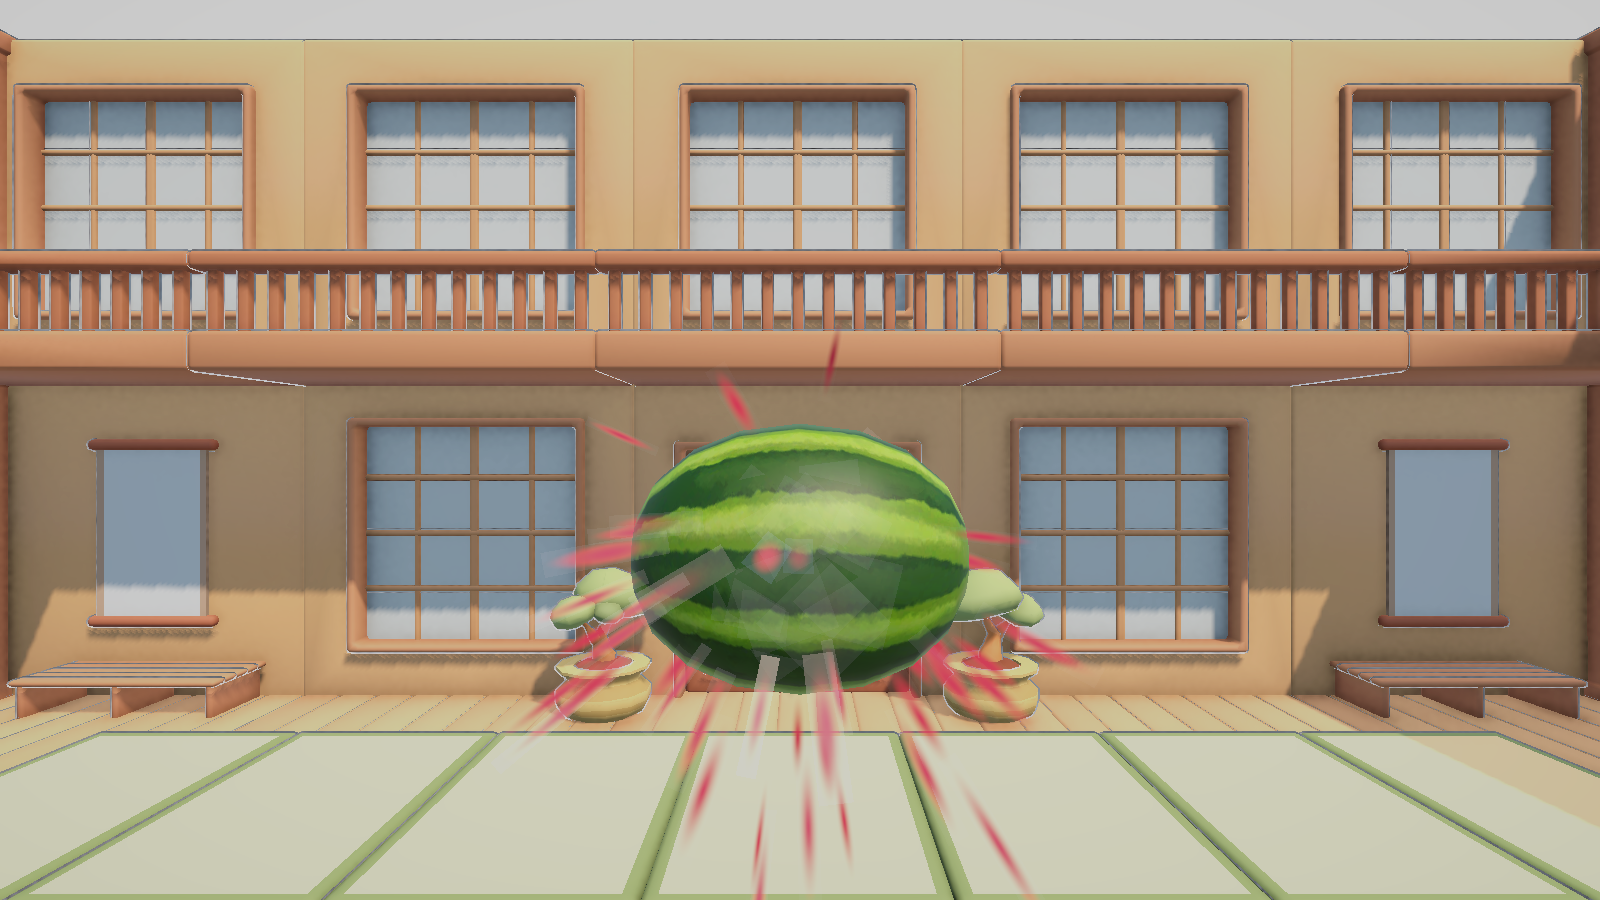
\includegraphics[width=0.38\textwidth]{FX_FruitJuice_PCVR.png} &
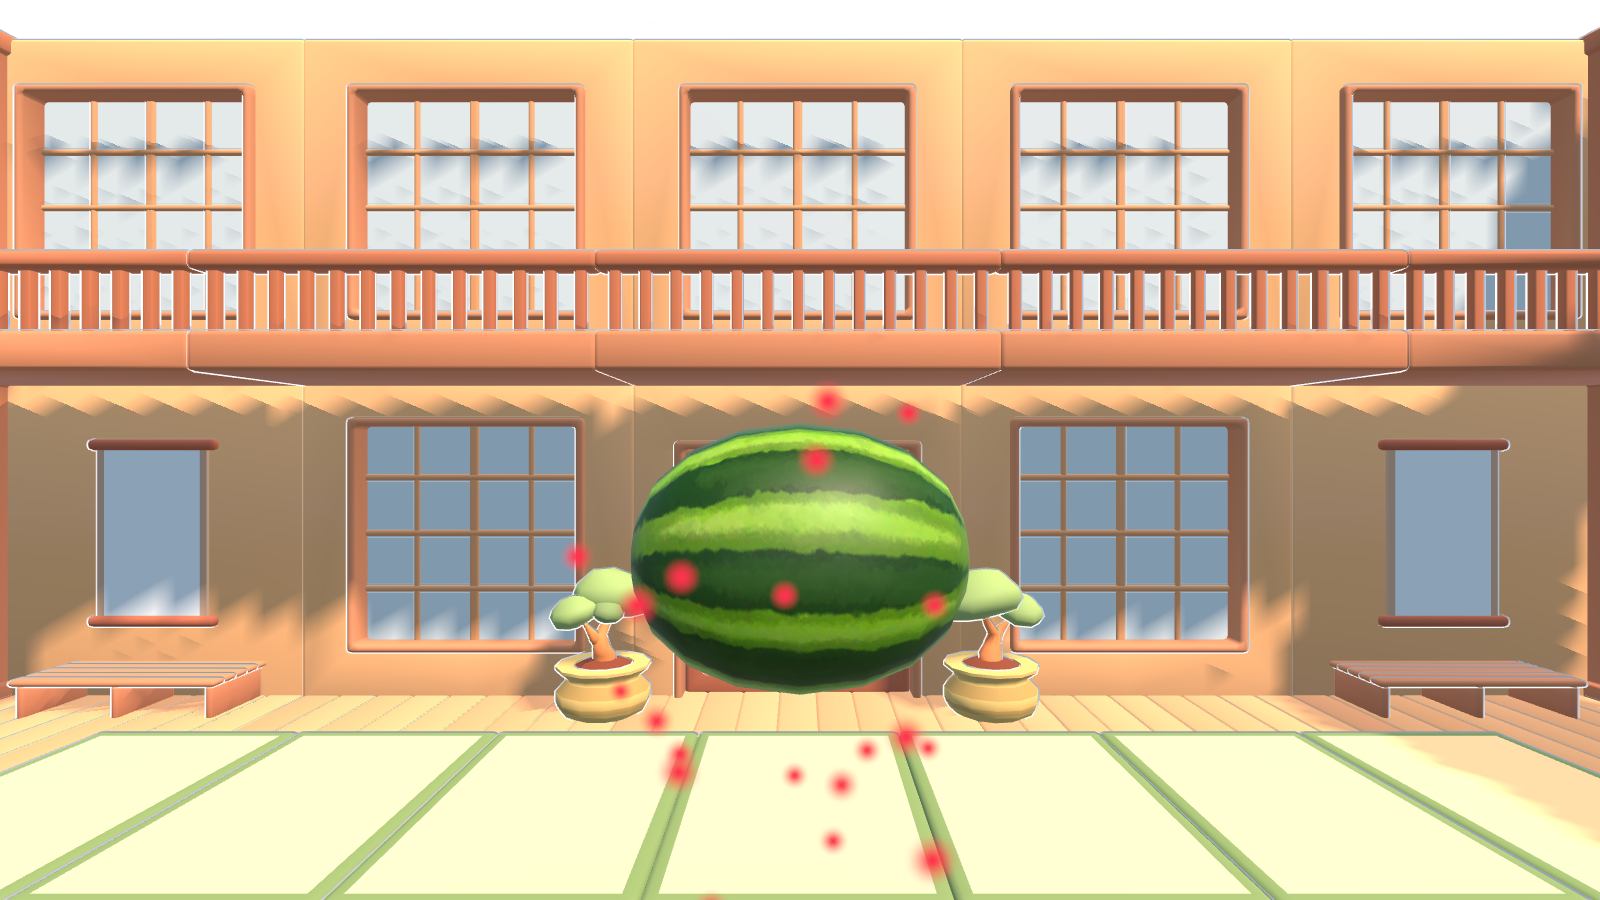
\includegraphics[width=0.38\textwidth]{FX_FruitJuice_Quest.png} \\
\small Jus -- PC (85 particules) & \small Jus -- Quest (20 particules) \\[4pt]
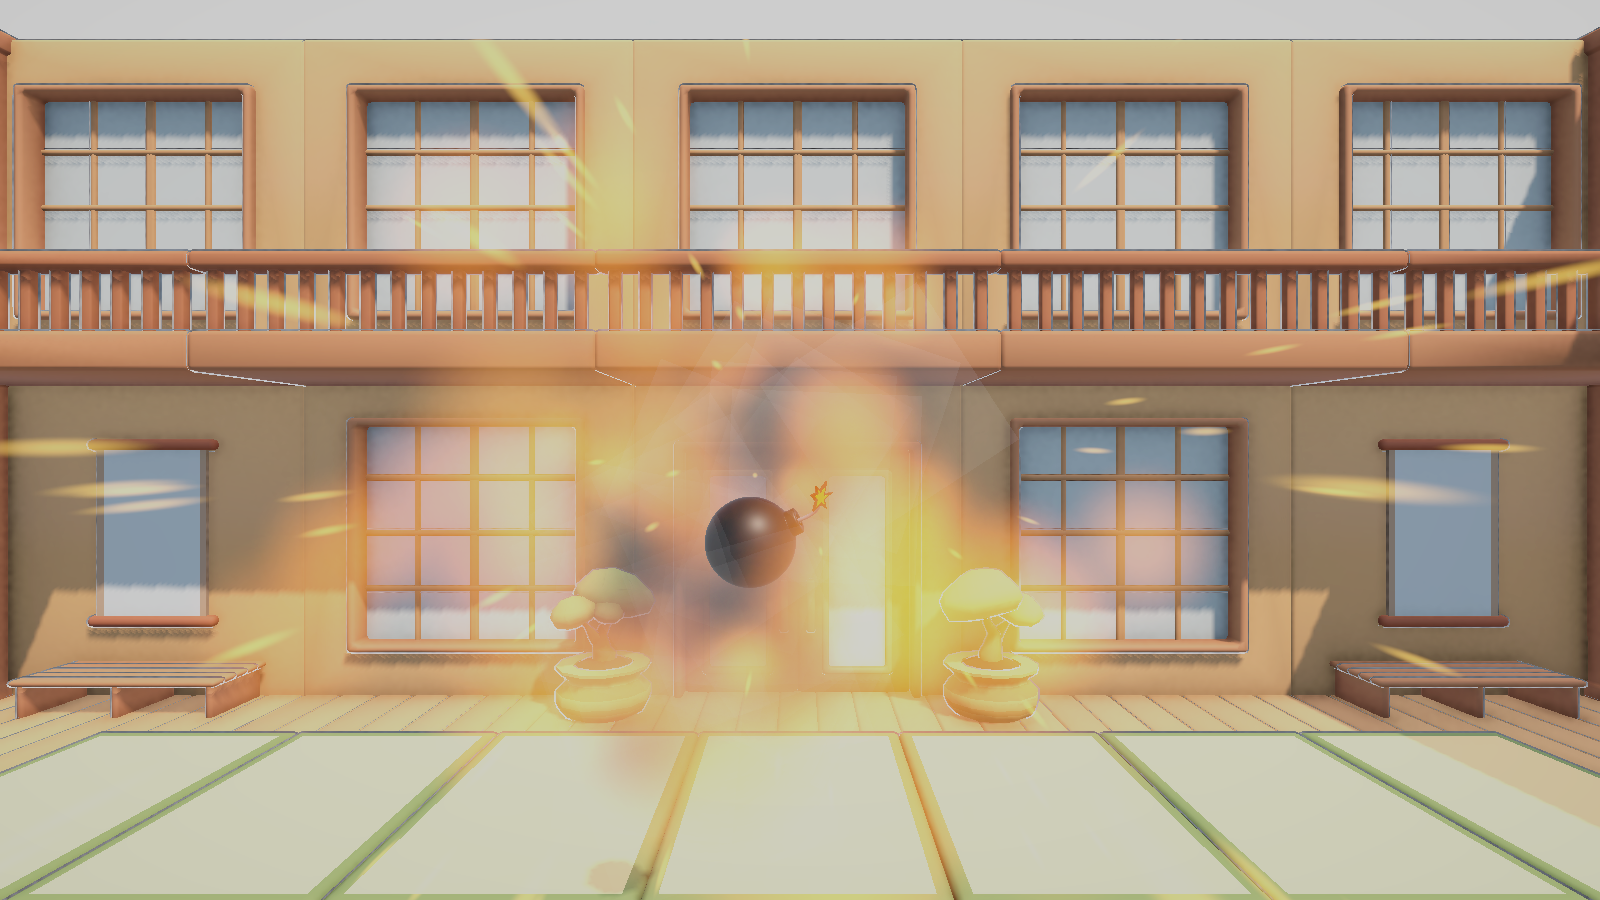
\includegraphics[width=0.38\textwidth]{FX_BombExplosion_PCVR.png} &
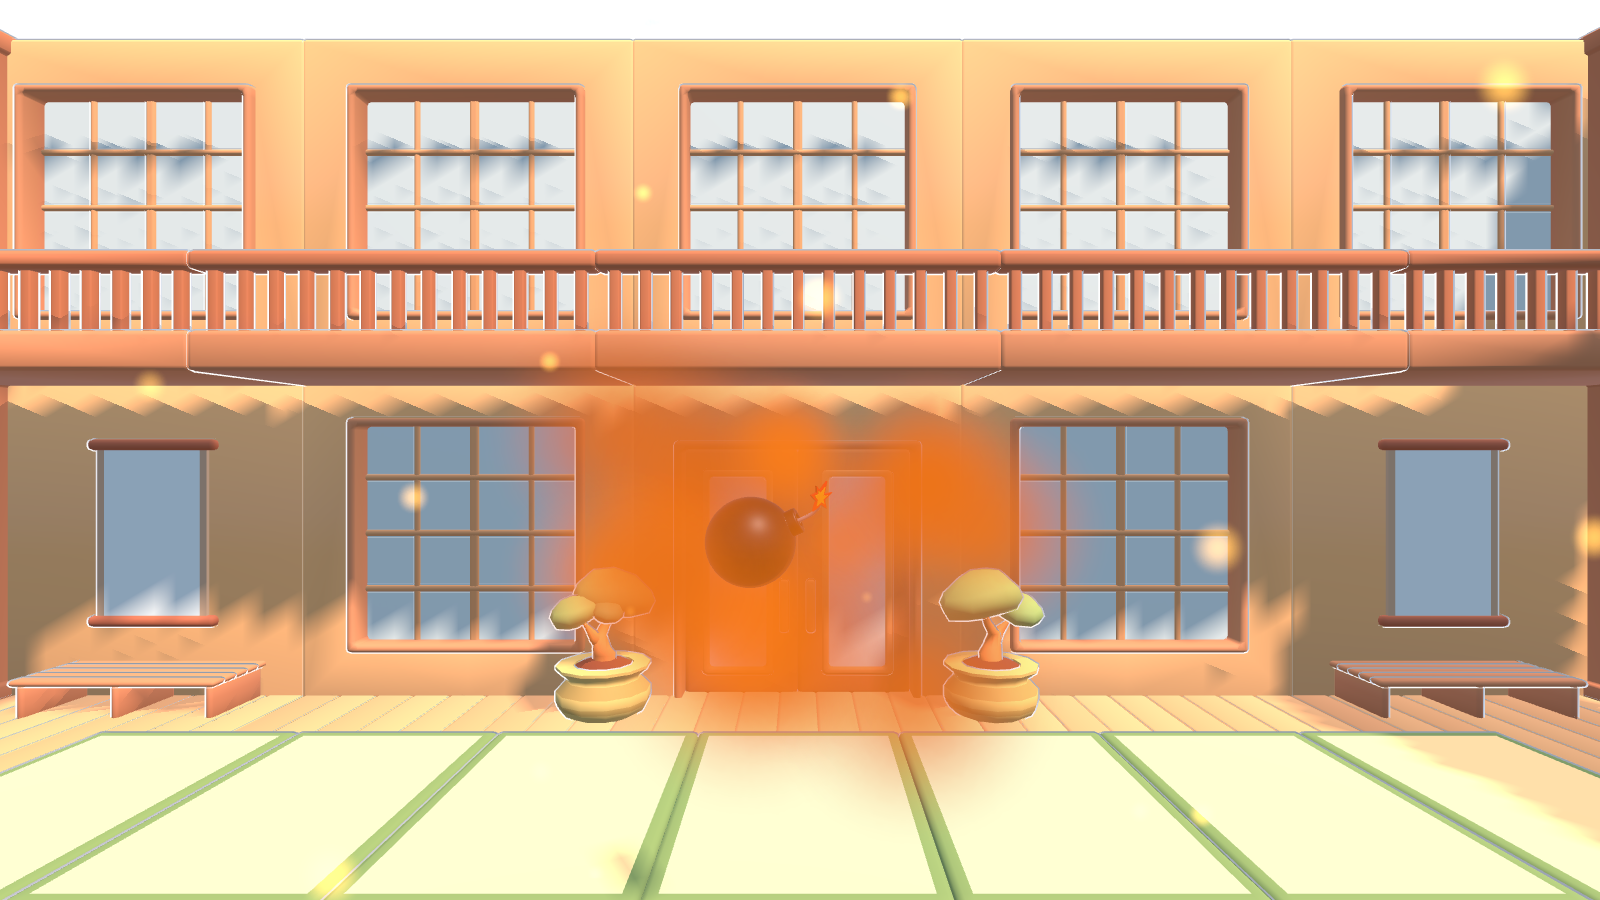
\includegraphics[width=0.38\textwidth]{FX_BombExplosion_Quest.png} \\
\small Explosion -- PC (185 particules) & \small Explosion -- Quest (40 particules) \\
\end{tabular}
\caption{Les deux effets rendus dans l'éditeur : PC à gauche, Quest à droite.}
\label{fig:fx}
\end{figure}

% =====================================================================
\section{Les builds et les tests au casque}

\paragraph{Réglages.} Un script construit les deux versions (menus \texttt{Tools > Fruit Ninja}).
\begin{itemize}
\item PC : Mono, x86\_64, Direct3D~11, textures BC, qualité \texttt{PC} (HDR, SSAO, ombres douces,
  post-process).
\item Quest : IL2CPP, ARM64 seul, Vulkan, textures ASTC, qualité \texttt{Mobile} (MSAA 4x, sans HDR ni
  post-process), API Android minimale 29, cible automatique (36).
\item Les deux : OpenXR, rendu Single Pass Instanced, Input System seul, scène \texttt{FruitNinjaVR\_Main}.
\end{itemize}

Les réglages Android du cours ne sont pas connus. On suit donc les recommandations de Meta et le profil
Meta Quest d'Unity 6. Il faudra les comparer à ceux du cours. Sur Android, on active OpenXR et Meta
Quest Support. On passe l'Input System en mode seul, car Android refuse le mode « Both ». On garde le
rig du S7 : il marche sur les deux plateformes, car OpenXR lui donne les positions dont il a besoin.
La validation OpenXR garde un seul avertissement (SSAO sur Android). C'est une fausse alerte : le
SSAO n'existe que dans le rendu PC.

\paragraph{Matériel.} PC sous Windows 11 (i9-14900KF, RTX 3080, 32 Go). Casque Meta Quest 3 sous Meta
Horizon OS v205 (Android 14), écran à 72~Hz. Pour le PC, Meta Horizon Link (runtime 1.208.0) par
câble USB-C.

\paragraph{Méthode.} Sur le Quest, il y a deux sessions. Dans la première, avec le câble, la
connexion adb coupe sans arrêt : Link utilise le même câble. On refait donc le test sans câble. On
agrandit le journal du casque avant de jouer, puis on le lit en rebranchant. Les captures par adb sont
noires. On utilise donc les captures du casque (bouton Meta + gâchette). Les FPS (images par seconde)
du Quest viennent du journal du casque : une ligne par seconde. Ceux du PC viennent du HUD de
performance de Link, capturé toutes les 2~s.

Le joueur répond « tout OK » sur les deux builds. La grille reprend ce retour. C'est du déclaratif.
La marque (j) indique ce que les journaux confirment aussi.

\begin{table}[!htb]
\centering\small
\caption{Grille de test résumée (OK : retour du joueur ; (j) : confirmé aussi par le journal).}
\begin{tabularx}{\textwidth}{@{}P{3.4cm}LP{2.0cm}P{2.0cm}@{}}
\toprule
Point & Ce qu'on vérifie & PC (Link) & Quest \\
\midrule
Démarrage & pas d'écran noir ni de crash & OK (j) & OK (j) \\
Tracking, katanas & tête, deux manettes, un katana par main & OK & OK \\
Menu & rayon et gâchette droite & OK & OK \\
Coupe, jus, combo & coupe nette, +10, jus coloré, combo +50, pomme dorée vue & OK (j) & OK (j) \\
Bombe touchée & $-25$ points, $-1$ vie, petite explosion & OK (j) & OK (j) \\
Explosion à 3 touches & tremblement, grande explosion, flash & non confirmée & non confirmée \\
Fin de partie, difficultés & écran de fin, vies selon le niveau & OK (j) & OK (j) \\
Lisibilité, fluidité & textes lisibles, pas de saccade & OK & OK \\
Stabilité & 2 parties sans crash & OK (j) & OK \\
Autonomie & jeu lancé sans câble ni PC & -- & OK (j) \\
\bottomrule
\end{tabularx}
\end{table}

Les journaux confirment la bonne version des effets sur chaque build (\texttt{[GameFX] variante
utilisée : Quest} et \texttt{: PCVR}). Ils ne montrent ni exception ni crash. L'explosion à 3 touches
n'apparaît dans aucun journal conservé : on n'y voit jamais plus de deux touches sur une même bombe.
Le parcours de test la prévoyait en Extrême. Or, en Extrême, on n'a qu'une vie : la partie s'arrête à
la première touche. Il faut la tester en Facile (5 vies).

\begin{figure}[!htb]
\centering
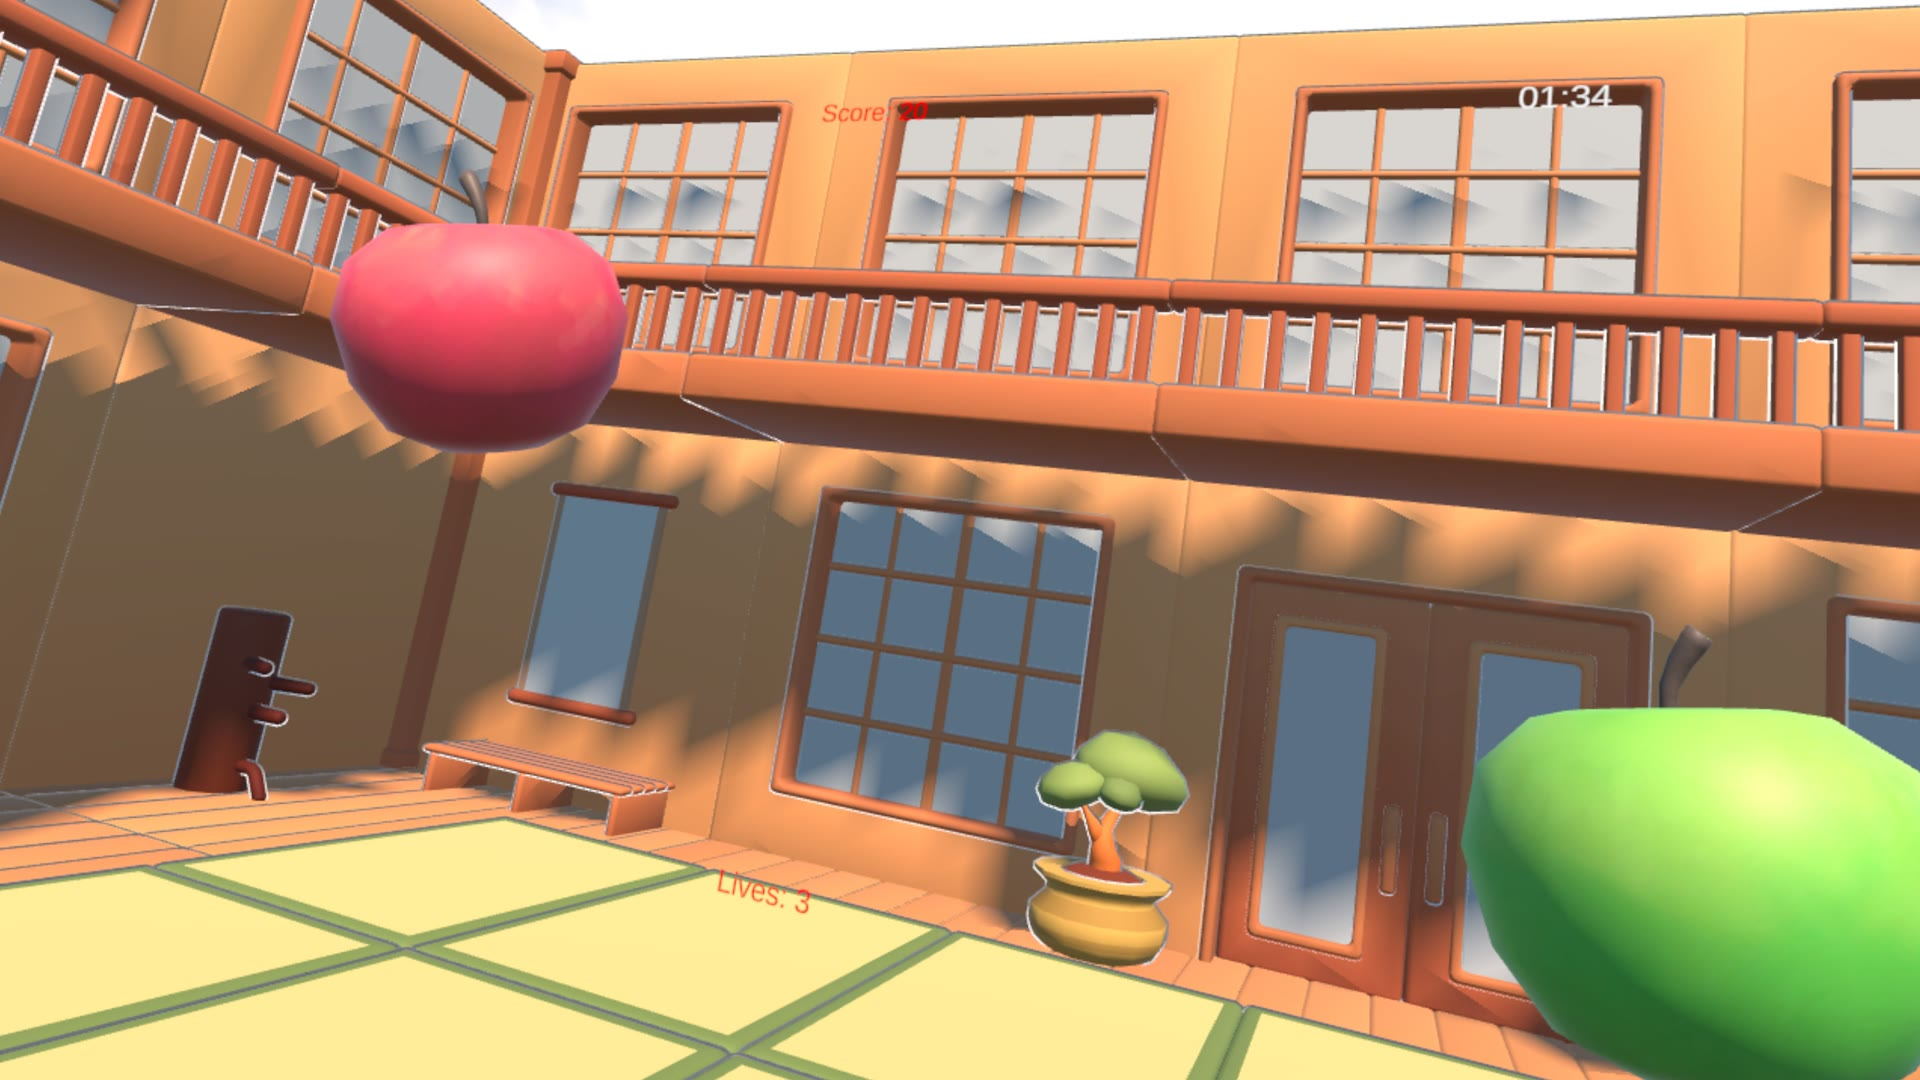
\includegraphics[width=0.48\textwidth]{quest/quest_jeu_fruits.jpg}
\caption{Capture dans le Quest 3 pendant une partie (vue d'un œil) : fruits, score, minuteur, vies.}
\label{fig:quest}
\end{figure}

\paragraph{Un bug trouvé grâce aux journaux.} Les deux journaux répètent l'erreur \texttt{Tag: Slice is
not defined} : 42 fois sur le Quest, 122 sur le PC. Elle vient du script \texttt{DestroyFloor} du S7.
Il teste les morceaux tombés au sol avec un tag qui n'existe pas. Rien ne se voit en jeu. On corrige
la ligne et on refait les deux builds. Les tests au casque ont donc eu lieu avant ce correctif. Le
nouvel APK est installé, mais pas relancé au casque. Son build se termine sans erreur.

% =====================================================================
\section{L'APK, les tailles et la fluidité}

\paragraph{Les tailles.} On ouvre l'APK dans l'APK Analyzer d'Android Studio. Il affiche
« APK size : 52.4 MB » et « Download Size : 47.4 MB ». Attention aux unités : ces « MB » sont des Mio
(1~Mio = $2^{20}$ octets). Le tableau, lui, est en Mo ($10^6$ octets). 52,4~Mio font bien 54,98~Mo. La
taille de téléchargement est une estimation de l'outil pour un store.

\begin{table}[!htb]
\centering\small
\caption{Tailles des builds finaux (1 Mo = $10^6$ octets).}
\begin{tabularx}{\textwidth}{@{}Lrr@{}}
\toprule
Fichier & Octets & Mo \\
\midrule
APK Quest & 54\,977\,835 & 54,98 \\
APK, taille de téléchargement estimée & 49\,709\,272 & 49,71 \\
Contenu de l'APK une fois décompressé & 149\,394\,197 & 149,39 \\
ZIP du build Windows & 71\,426\,270 & 71,43 \\
Dossier Windows livré & 152\,105\,649 & 152,11 \\
\bottomrule
\end{tabularx}
\end{table}

Un APK est déjà une archive ZIP. On le compare donc au ZIP Windows. On compare aussi son contenu
décompressé au dossier Windows. L'APK réduit ses données à 36,8~\% de leur taille. Le ZIP Windows
seulement à 47,0~\%. En effet, les textures PC sont déjà très compactes. Et le build Windows contient
en plus le moteur (\texttt{UnityPlayer.dll}) et les bibliothèques .NET.

Les captures de l'APK Analyzer viennent d'un build de la veille. Depuis, l'APK a changé de 224 octets
seulement. Les valeurs arrondies ne bougent pas. Le dossier Windows a perdu 0,73~Mo. Un outil de
développement (MCP for Unity) se retrouvait en partie dans le build PC. On le retire avant la remise.

\begin{figure}[!htb]
\centering
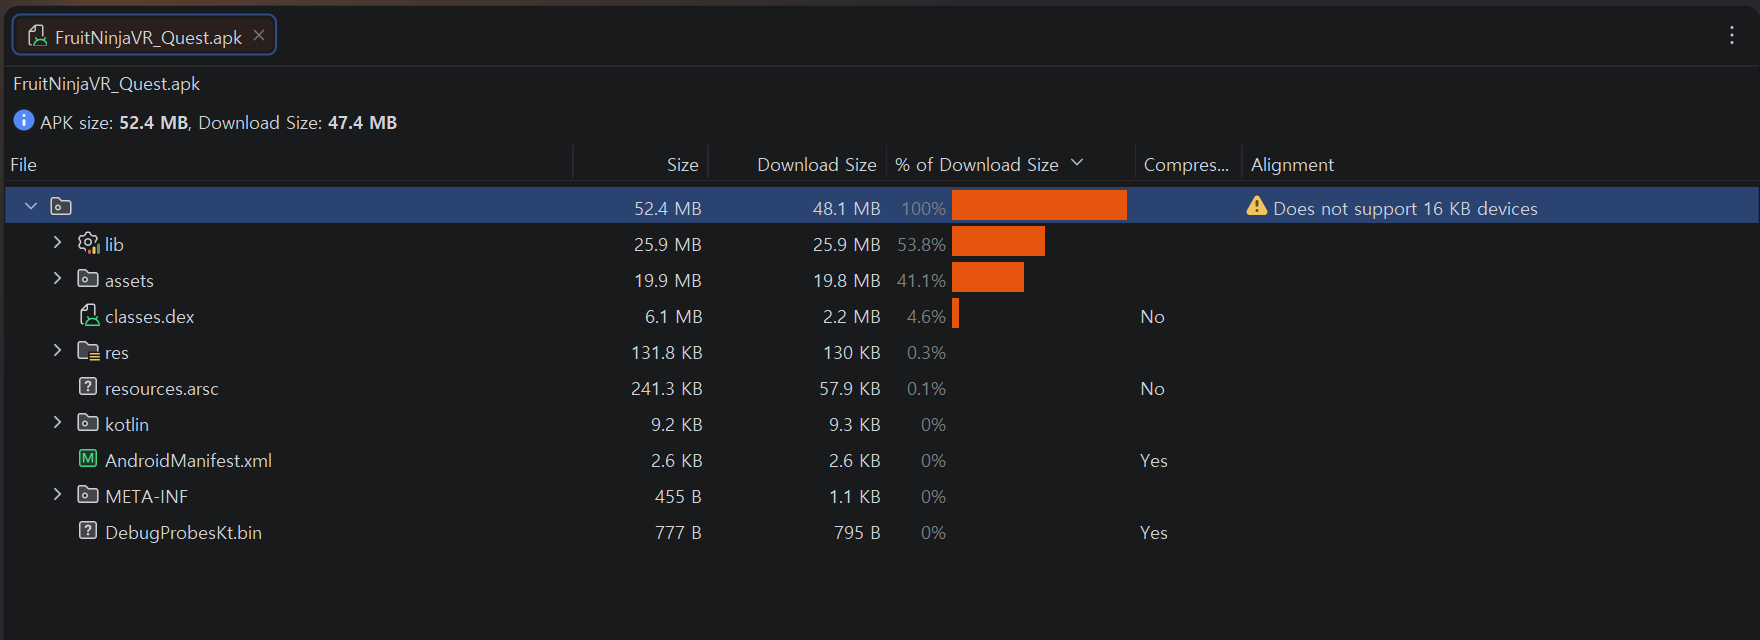
\includegraphics[width=0.72\textwidth]{apk-analyzer/01-vue-ensemble.png}
\caption{APK Analyzer : le code natif (\texttt{lib}) fait 53,8~\% du téléchargement, les données Unity
(\texttt{assets}) 41,1~\%.}
\label{fig:apk}
\end{figure}

\paragraph{Ce qui prend de la place.}
\begin{itemize}
\item Le code natif, environ la moitié de l'APK. \fichier{libil2cpp.so} pèse 16,2~Mo compressé
  (64,8~Mo décompressé). Il contient tout le C\# des paquets (XR Interaction Toolkit, Input System,
  URP\ldots), pas seulement les scripts du jeu. IL2CPP le traduit en C++. Le \emph{stripping}
  (suppression du code inutilisé) est sur « Minimal ». Plus fort, il réduirait ce fichier, mais
  risquerait de retirer du code utile aux paquets.
\item Le moteur (\fichier{libunity.so}) : 9,5~Mo.
\item Les textures : 73,5~\% des assets du jeu sur Android. La plus grosse est le ciel HDR en 4K :
  14,3~Mo en ASTC sur le Quest, contre 32,0~Mo en BC6H sur PC.
\item Les meshes, les shaders et les sons pèsent peu.
\end{itemize}
L'outil affiche aussi « Does not support 16 KB devices ». Cela vient des deux bibliothèques OpenXR des
paquets. On ne peut pas les modifier dans le projet. Aucun effet n'est constaté sur le Quest 3, mais
c'est à surveiller.

\paragraph{La fluidité.} Les deux builds tiennent les 72 images par seconde de l'écran. La différence
est dans la marge qui reste.

\begin{table}[!htb]
\centering\small
\caption{FPS mesurés en jeu (écran à 72~Hz).}
\begin{tabularx}{\textwidth}{@{}P{2.5cm}P{1.6cm}P{1.7cm}L@{}}
\toprule
Build, partie & Moyenne & Minimum & Remarques \\
\midrule
Quest, Normal & 72,5 & 71 & 85~s, aucune seconde sous 70 ; GPU occupé à 81~\% (88~\% au plus), CPU à 23~\% \\
Quest, Extrême & -- & -- & non mesuré (journal de la 1\textsuperscript{re} session perdu) \\
PC, Normal & 72,0 & 72 & 38~s mesurées, 1 image perdue ; marge de 77 à 84~\% \\
PC, Extrême & 72,0 & 72 & environ 40~s, aucune image perdue ; marge de 71 à 85~\% \\
\bottomrule
\end{tabularx}
\end{table}

Sur le Quest, la moyenne de 72,5 dépasse 72 à cause du découpage des secondes par le compteur. Le GPU
met 9,4~ms par image (10,0~ms au plus). Le budget est de 13,9~ms à 72~Hz. Il reste donc environ
28~\% de marge. C'est le GPU qui limite, pas le CPU. Alléger les particules était donc utile. La seule
baisse vient du chargement : une seconde à 64~FPS, juste avant le menu.

Sur le PC, la RTX 3080 garde 71 à 85~\% de marge. Le seul creux (63~Hz) a lieu au retour au menu,
hors partie. Le PC pourrait afficher les effets complets. Le Quest a besoin de la version allégée.

À l'œil, les deux versions ont le même décor et la même interface. Le PC a en plus l'éclairage HDR, le
post-process et des jus plus fournis. Le Quest est plus plat, mais les effets restent lisibles. Le
joueur ne signale ni saccade ni texte illisible. Via Link, la latence entre le geste et l'image est
d'environ 43~ms. Elle vient du streaming et n'existe pas en autonome.

% =====================================================================
\section{Difficultés, limites et bilan}

\paragraph{Difficultés.}
\begin{itemize}
\item Le build Android échoue (« Failed to update Android SDK »). Cause :
  \fichier{C:\textbackslash Windows\textbackslash System32} manque dans le PATH du poste, donc
  la commande \texttt{findstr} est introuvable. On lance Unity avec un PATH corrigé. Le PATH du poste
  reste à réparer.
\item Le SDK Android 32 demandé n'est pas installé. Le SDK d'Unity, dans \fichier{Program Files}, ne
  se modifie pas sans droits administrateur. On règle donc la cible sur « Automatic », soit l'API 36.
\item Pendant les tests : connexion adb coupée par Link, journal du casque trop petit (256~Kio, écrasé
  en quelques minutes), captures adb noires. Les solutions sont décrites en partie 3.
\end{itemize}

\paragraph{Limites.}
\begin{itemize}
\item La grande explosion à 3 touches n'est pas confirmée par les journaux.
\item Les FPS du Quest en Extrême ne sont pas mesurés.
\item Le dernier APK (avec le correctif de \texttt{DestroyFloor}) est installé, mais pas relancé au casque.
\item Le bouton Quitter du menu réagit au contact des katanas. Pendant le test PC, le jeu s'est fermé
  après un retour au menu.
\item Volume, mode entraînement, classement et sauvegarde JSON restent absents, comme au S7.
\item Le rig legacy du S7 est conservé.
\item Les réglages Android sont à comparer à ceux du cours.
\item Des objets de test et des \texttt{Debug.Log} restent dans la scène.
\item Le ciel HDR en 4K est le premier poste à réduire si la taille ou la mémoire posent problème.
\end{itemize}

\paragraph{Conclusion.} Ce projet a permis de voir qu'il faut mesurer sur le casque plutôt que
deviner. Le Quest tient 72~FPS, mais avec environ 28~\% de marge seulement, et c'est le GPU qui
limite. Sans les effets allégés, cette marge aurait fondu. Le projet a aussi montré pourquoi on
déplace les assets depuis l'éditeur, et qu'une taille d'APK se lit avec ses unités, en comparant des
archives entre elles. Enfin, les journaux ont été très utiles : ils ont révélé le bug du tag
\texttt{Slice}, invisible en jeu.

\paragraph{Ce qu'on referait autrement.} On préparerait les mesures avant de jouer : journal du casque
agrandi dès le début, HUD de Link prêt. On prévoirait un test pour chaque point, par exemple
l'explosion à 3 touches en Facile. On ferait tous les tests sur le build final, pour ne laisser aucun
correctif non vérifié au casque. Enfin, on retirerait plus tôt les outils de développement, car l'un
d'eux s'était glissé dans le build PC.

\end{document}
